\documentclass[11pt,handout]{beamer}
\usetheme{Warsaw}
\usepackage[utf8]{inputenc}
\usepackage[french]{babel}
\usepackage[T1]{fontenc}
\usepackage{amsmath}
\usepackage{amsfonts}
\usepackage{amssymb}
\usepackage{graphicx}
\hypersetup{pdfpagemode=FullScreen}
\author[Ramadan SOUMAILA]{}
\title{Système de géolocalisation sur le campus d'Abomey-Calavi}
\setbeamercovered{transparent} 
%\setbeamertemplate{navigation symbols}{} 
\logo{} 
\institute{} 
\date{} 
%\subject{}
\AtBeginSection[]
{
\begin{frame}
\transdissolve[duration=1]
\frametitle{Sommaire}
\tableofcontents[currentsection,hideallsubsubsections]
\end{frame}
} 
\begin{document}
\begin{frame}
	\begin{center}
	
\includegraphics[scale=0.15]{images/logoUAC1.png}
	 \hspace{1.1cm}
	  {\scriptsize \textbf{\textsf{UNIVERSITÉ D'ABOMEY-CALAVI}}}
	   \hspace{1.1cm}
	   
\includegraphics[scale=0.15]{images/logoIfri.png}\\
	  {\footnotesize \textbf {\textsf{INSTITUT DE FORMATION ET DE RECHERCHE EN INFORMATIQUE}}}
	\end{center}
	\begin{center}
		\titlepage
		Présenté par : Ramadan \textbf{SOUMAILA\\}
		Sous la supervision de : Prof Eugène C. \textbf{EZIN}
	\end{center}
\end{frame}
\begin{frame}
\frametitle{Plan}
\tableofcontents
\end{frame}
	\section{Contexte et Problématique}
		\subsection{Problématique}
			\begin{frame}
			    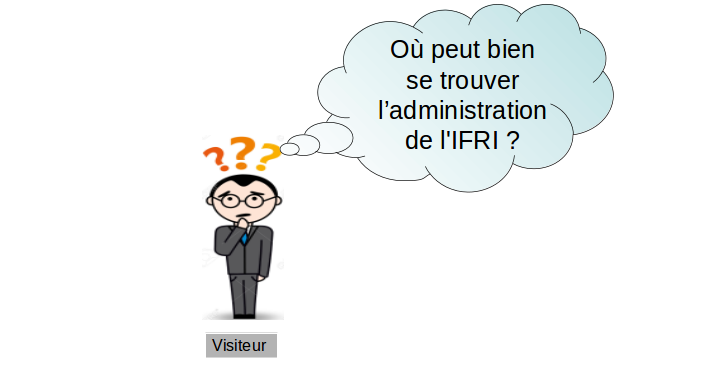
\includegraphics[scale=0.5]{images/problematique_1.png}
			\end{frame}
			\begin{frame}
			    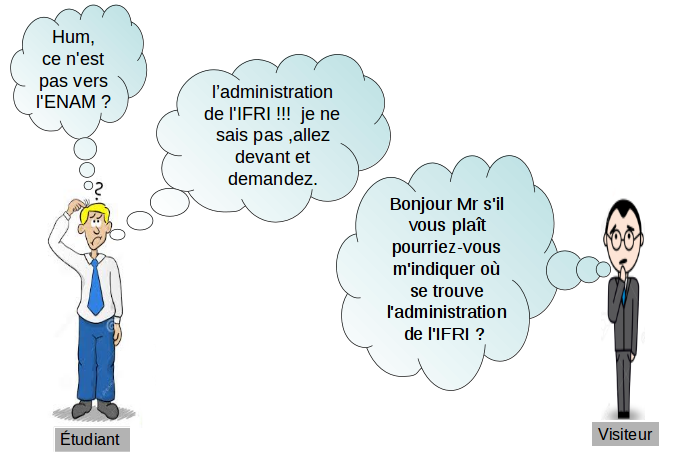
\includegraphics[scale=0.45]{images/preuve_2.png}
			\end{frame}
		\subsection{Objectifs}
			\begin{frame}
			\begin{exampleblock}{Objectif principal}
			      Faciliter et rendre autonomes les déplacements au sein de l'UAC.
			\end{exampleblock}
			  \begin{exampleblock}{Objectifs spécifiques}
			    \begin{itemize}
			    \setbeamertemplate{itemize item}[square]
			     \item se géolocaliser.
			     \item calculer un itinéraire.
			     \item rechercher un bâtiment.
			     \item consulter la fiche d'un bâtiment.
			     \item utiliser la navigation.
			    \end{itemize}
			  \end{exampleblock}
			\end{frame}
		\subsection{Organisation du mémoire}
			\begin{frame}
			      \begin{block}{Organisation du mémoire}
			      \begin{enumerate}
			       \item Revue de littérature.
			       \item Conception et Matériels.
			       \item Résultats et discussion.
			      \end{enumerate}
			      \end{block}
			\end{frame}
	\section{Revue de littérature}
		\subsection{Généralités sur la géolocalisation}
			\begin{frame}
			\begin{center}
			  \begin{Huge}
			      \textbf{Qu'est ce que la géolocalisation ?}
			  \end{Huge}
			  \end{center}
			\end{frame}
			\begin{frame}
			    \begin{definition} % Définition
			  \emph{«technique de détermination de la situation géographique précise d’un lieu ou, à un instant donné, d’une
			      personne, d’un véhicule, d’un objet, etc»}.
			    \end{definition}
			    \begin{block}{Ce qu'il faut retenir}
				La géolocalisation est donc un procédé permettant de positionner à un instant donné un objet
			    sur un plan ou une carte à l’aide de ses coordonnées géographiques obtenues en utilisant une
			    technique de localisation.
			    \end{block}
			\end{frame}
			    \begin{frame}
				 \begin{block}{Les Techniques de localisation}
				      \begin{itemize}
				      \setbeamertemplate{itemize item}[square]
				       \item Triangulation de satelittes.
				       \item Identifiant de cellule (CellID).
				       \item Angle d'arrivée (AoA).
				       \item Differencielle de Temps d'arrivée (TDOA).
				       \item Puissance de signal reçue (RSS).
				      \end{itemize}
				 \end{block}
			    \end{frame}
			    \begin{frame}
				 \begin{block}{Les Types de géolocalisation}
				      \begin{itemize}
				      \setbeamertemplate{itemize item}[square]
				       \item la géolocalisation par satelittes.
				       \item la géolocalisation par WIFI.
				       \item la géolocalisation par GSM.
				       \item la géolocalisation par RFID.
				       \item la géolocalisation par IP.
				       \item la géolocalisation par géocodeur.
				      \end{itemize}
				 \end{block}
			    \end{frame}
		\subsection{Solutions existantes}
			\begin{frame}
			    \begin{exampleblock}{Solutions existantes}
				\begin{itemize}
				 \setbeamertemplate{itemize item}[square]
				 \item Google Maps.
				 \item OpenStreetMap.
				\end{itemize}
			    \end{exampleblock}
			    \begin{block}{Fonctionnalités}
				\begin{itemize}
				 \item Trouver la position de l'utilisateur.
				 \item Calculer un itinéraire.
				 \item Effectuer la navigation.
				 \item etc...
				\end{itemize}
			    \end{block}
			     \begin{alertblock}{Insuffisance}
			      Aucune d'elles ne présente le plan de l'UAC.
			  \end{alertblock}
			\end{frame}		
	\section{Conception et Matériels}
		\subsection{Conception}
			\begin{frame}
			  \frametitle{Méthode de modélisation}
				Langage de modélisation orienté objet : Unified Modeling Language (UML)\\
				Diagrammes réalisés :
				\begin{itemize}
				 \setbeamertemplate{itemize item}[square]
				 \item Diagramme des cas d'utilisations.
				 \item Diagramme de séquences.
				\end{itemize}
			\end{frame}
			\begin{frame}
			    \begin{block}{Diagramme des cas d'utilisations}
			      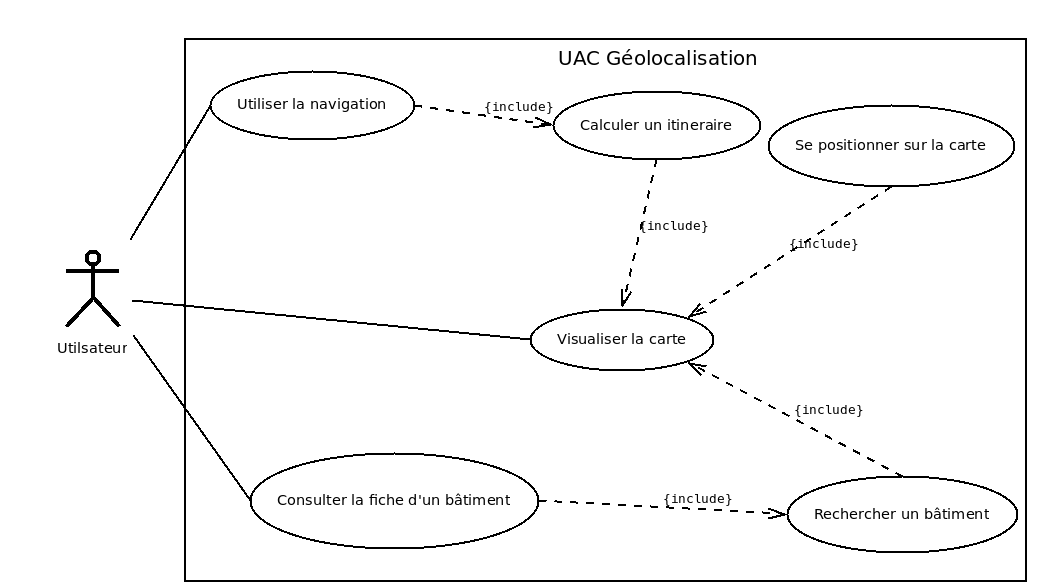
\includegraphics[scale=0.3]{images/cas_utilisation.png}
			    \end{block}
			\end{frame}
			\begin{frame}
			    \begin{block}{Diagramme de séquence :Rechercher un bâtiment}
			      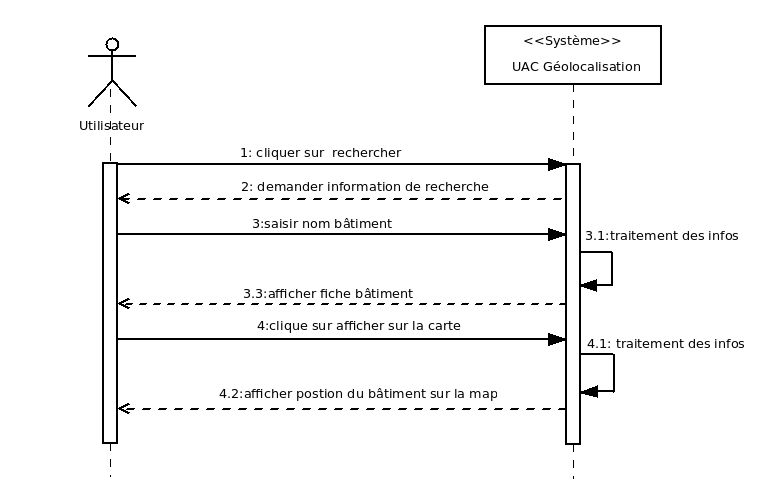
\includegraphics[scale=0.4]{images/sequence_batiment.png}
			    \end{block}
			\end{frame}
			\begin{frame}
			    \begin{block}{Diagramme de séquence :Calculer un itinéraire}
			      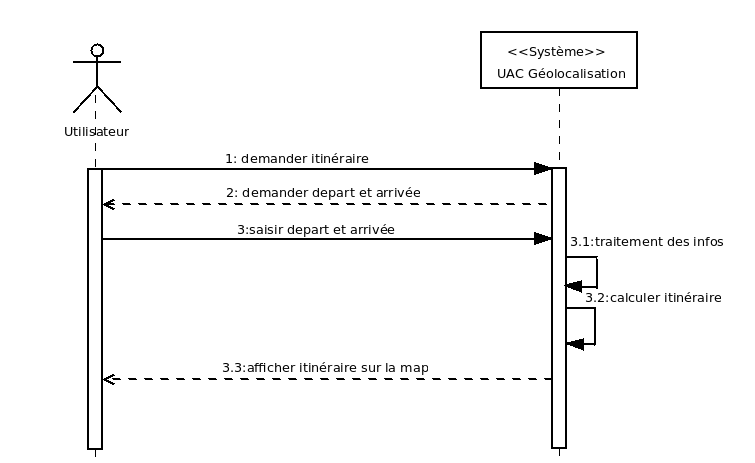
\includegraphics[scale=0.4]{images/sequence_itineraire.png}
			    \end{block}
			\end{frame}
		\subsection{Matériels}
			\begin{frame}
			      \begin{block}{Principe de fonctionnement de notre solution}
				  \begin{enumerate}
				   \item intégrer le plan de l'UAC sur OpenStreetMap.
				   \item développement de l'application.
				  \end{enumerate}
			      \end{block}
			      \begin{block}{Langages}
				  \begin{itemize}
				   \item JAVA.
				   \item XML. 
				  \end{itemize}
			      \end{block}
			      \pause
			      \begin{block}{Logiciels}
				  \begin{itemize}
				   \item JDK 8 .
				   \item Android Studio 1.2.2 .
				   \item SDK 22.0 (Android 5.0) .
				   \item JOSM 8339 .
				  \end{itemize}
			      \end{block}
			\end{frame}
	\section{Présentation de UAC Géolocalisation}

	\section{Conclusion et perspectives}
			\begin{frame}
			\begin{center}
			  \begin{Huge}
			      \textbf{Conclusion }
			  \end{Huge}
			  \end{center}
			\end{frame}
			\begin{frame}
			    \begin{block}{Perspectives}
				\begin{itemize}
				\setbeamertemplate{itemize item}[square]
				 \item rendre l'application accessible sur d'autres plâteformes telles que iOS de Apple ou RIM de Blackberry. 
				 \item possibilité d'utiliser l'application en mode hors ligne.
				\end{itemize}
			    \end{block}
			\end{frame}
\section*{}
    \begin{frame}
	\begin{center}
		\begin{Huge}
		      \begin{center}
		       \textbf{MERCI}
		      \end{center}
		       \begin{center}
		       \textbf{POUR}
		      \end{center}
		      \begin{center}
		       \textbf{VOTRE}
		      \end{center}
		      \begin{center}
		       \textbf{ATTENTION !!!}
		      \end{center}
		\end{Huge}
	\end{center}
\end{frame}

%\begin{frame}
%\tableofcontents
%\end{frame}


\end{document}